\documentclass{article}
    \usepackage{amssymb}
    \usepackage[utf8]{inputenc}
    \usepackage[russian]{babel}
    \usepackage[left=2cm,right=2cm,
        top=2cm,bottom=2cm,bindingoffset=0cm]{geometry}
    \usepackage{hyperref}
    \hypersetup{
        colorlinks=true,
        linkcolor=blue,
        filecolor=magenta,      
        urlcolor=cyan,
    }
  \usepackage{graphicx}
  \usepackage{booktabs}
  \usepackage{hyperref}
  \graphicspath{{pictures/}}
  \DeclareGraphicsExtensions{.pdf,.png,.jpg}
\usepackage{subcaption}
%\captionsetup{compatibility=false}

\begin{document}
\begin{center}{\hugeОтчет по дипломной работе за неделю\\}\end{center}
Дата: 18.3.2021\\
Научные руководители: Герасимов С.В., Мещеряков А.В.\\
Студент: Немешаева Алиса\\
Курс: 4\\

\renewcommand{\labelitemi}{$\blacksquare$}
\renewcommand\labelitemii{$\square$}
\begin{enumerate}
    %\item Добавлена иллюстрация модели Unet для статьи. 
    %    ~\ref{Fig:Unet}{}\\
    \item Прочитана  \href{https://arxiv.org/pdf/2102.13123.pdf}{статья}, по ней было проведено 
        обсуждение.\\
    \item Исправлены иллюстрации в презентации (заменены на более актуальные):
        \begin{itemize}
            \item График обучения для лучшей модели. ~\ref{Fig:Hist}{}\\
            \item Карта каталога ACT. ~\ref{Fig:ACT}{}\\
            \item Сопоставление с каталогом eROSITA. ~\ref{Fig:Erosita}\\ 
            \item Сопоставление brcat с PSZ2, ACT, MCXC, RM. ~\ref{Fig:Brcat}{}\\
            \item Статистика по патчам. ~\ref{Fig:Patches}{}\\
        \end{itemize}
\end{enumerate}




\begin{figure}[h]
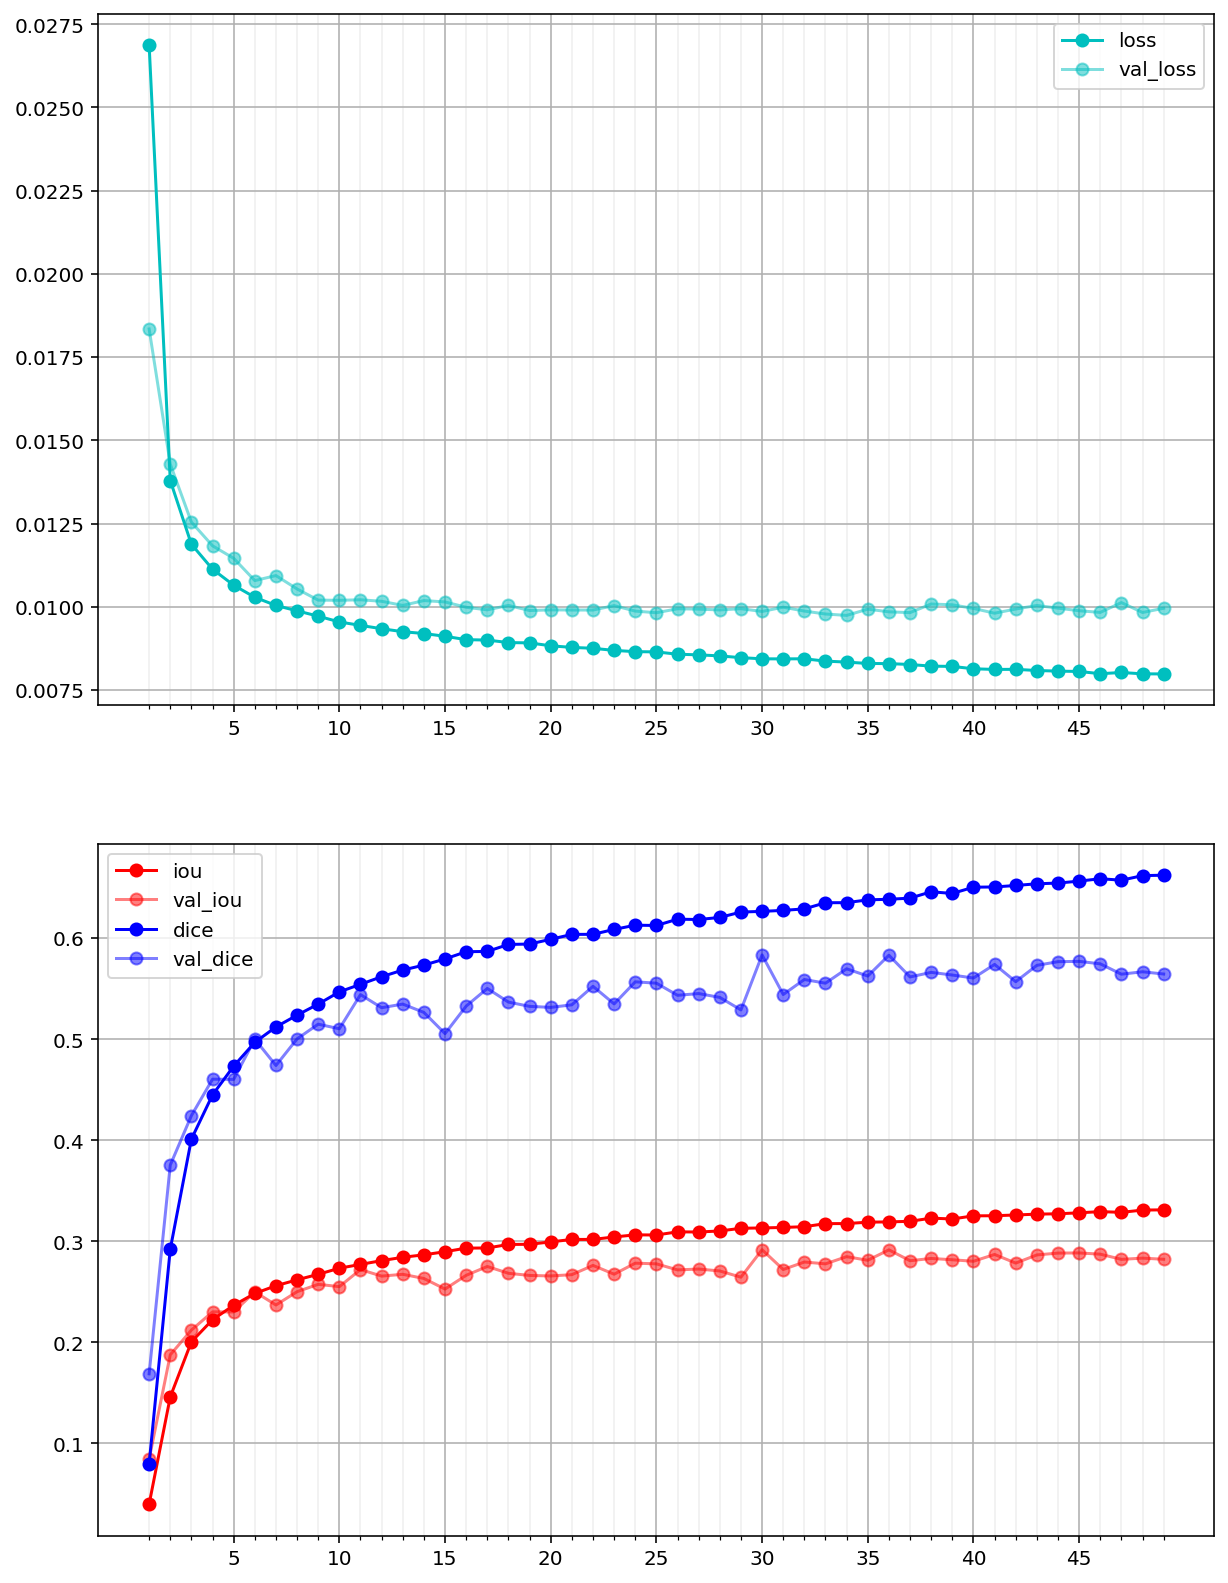
\includegraphics[width=0.6\linewidth]{all_found_hist}
\caption{График обучения модели pz\_all\_found}
\label{Fig:Hist}
\end{figure}

\begin{figure}[h]
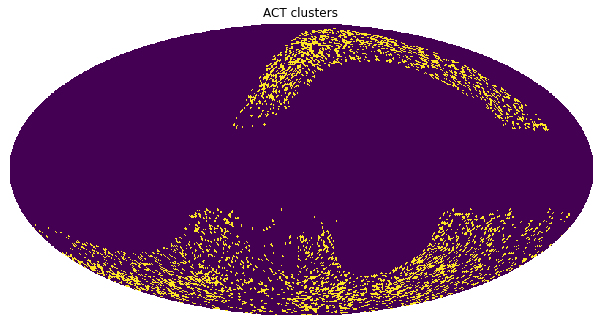
\includegraphics[width=0.6\linewidth]{act_map}
\caption{Распределение скоплений ACT}
\label{Fig:ACT}
\end{figure}

\begin{figure}[h]
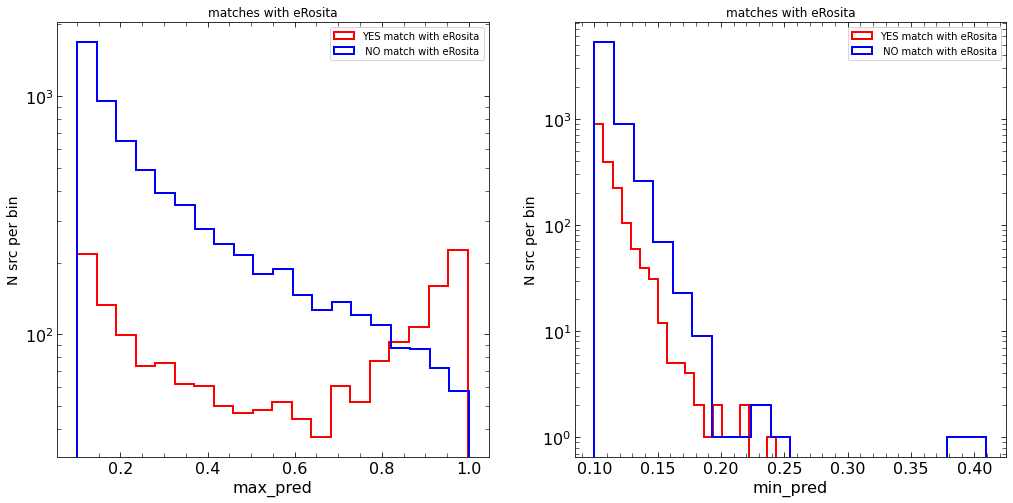
\includegraphics[width=0.8\linewidth]{ancat_erosita_histogram}
\caption{Сопоставление каталога pz\_all\_found с eROSITA по max\_pred}
\label{Fig:Erosita}
\end{figure}

\begin{figure}[h]
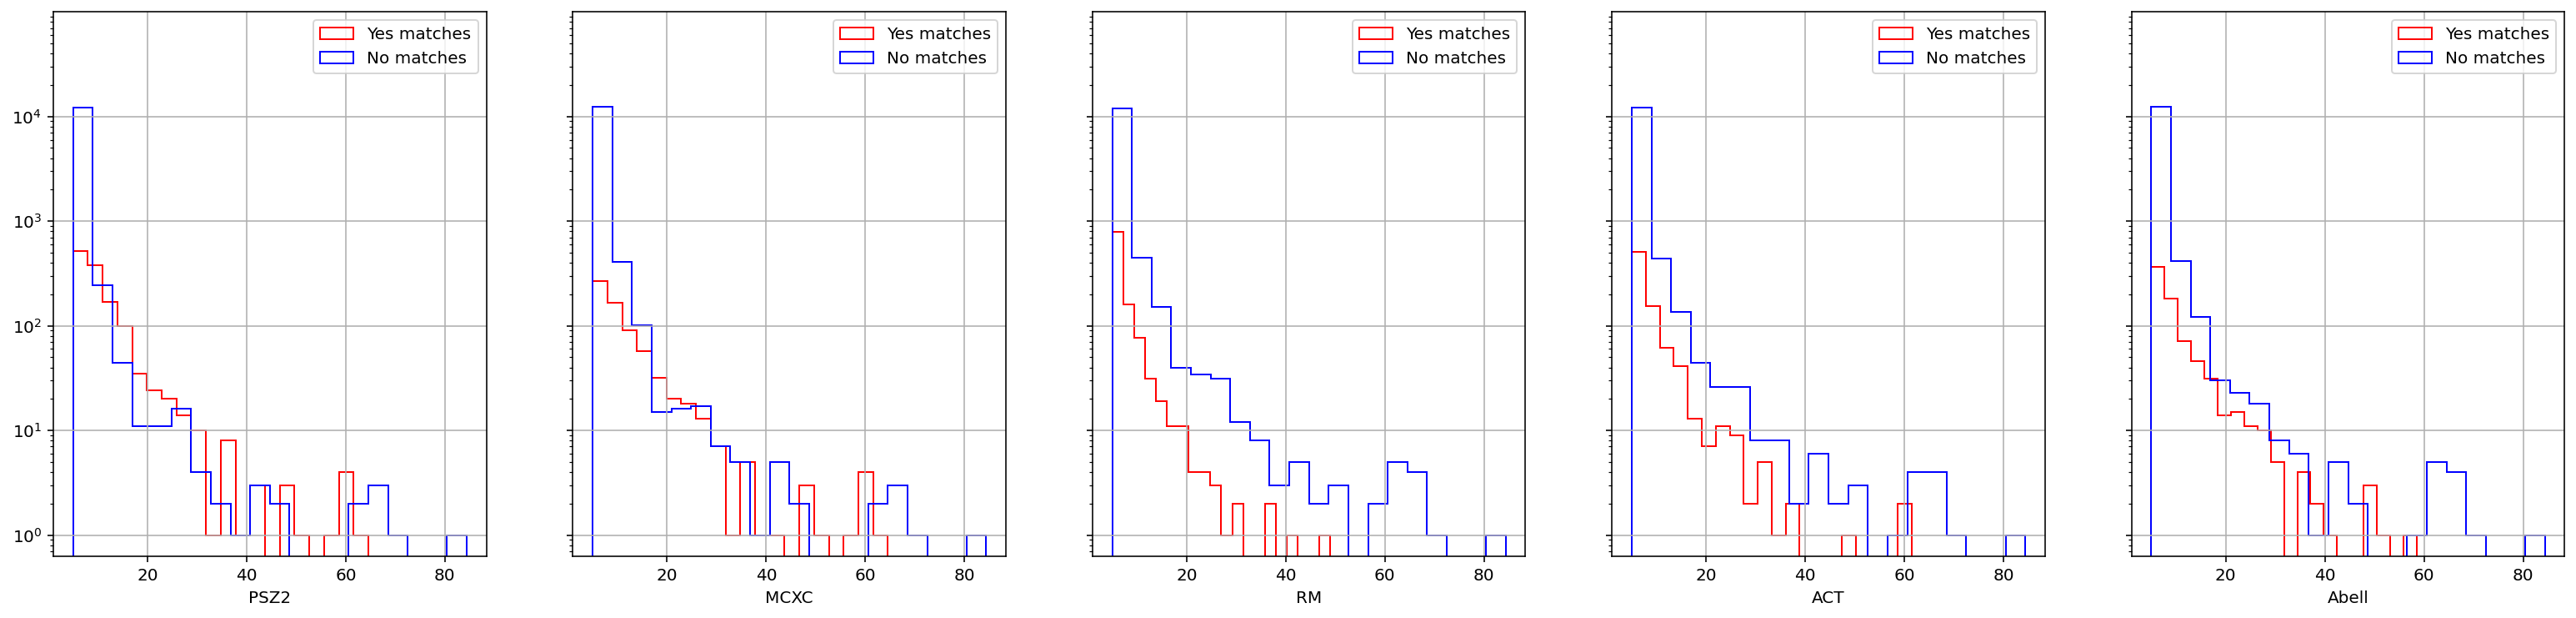
\includegraphics[width=0.8\linewidth]{brcat_histogram}
\caption{Сопоставление brcat с PSZ2, ACT, MCXC, RM.}
\label{Fig:Brcat}
\end{figure}

\begin{figure}[h]
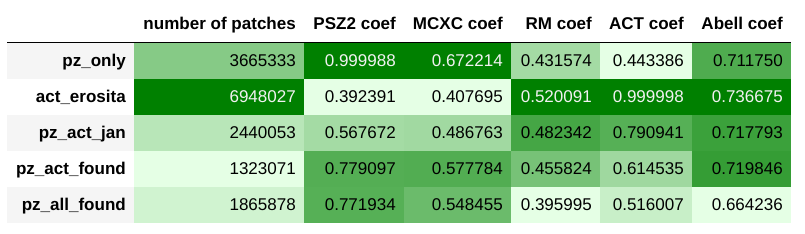
\includegraphics[width=0.6\linewidth]{patch_stat}
\caption{Статистика списков с патчами по каталогам. Число в колонке по каталогу означает вероятнось,
    с которой патч из списка содержит скопление из каталога колонки.}
\label{Fig:Patches}
\end{figure}
Отчет согласован с научным руководителем.\\
Общее количество строк кода за эту неделю: 102\\
\href{https://github.com/rt2122/data-segmentation-2}{Репозиторий}\\ 
\end{document}
